\section{Signal Studies}
\label{sec:signal}
The various properties of the \HToZg signal are described in this section.
This includes a discussion of the number of signal events expected to be
observed in data (expected signal yield) followed by a description
of the template model used to describe the signal's shape in data.

\subsection{Expected signal yield}
An understanding of the expected signal yield follows the same calculation
described in \refS{subsec:prodproc} with an additional term that accounts
for the fact that the selection described in \refS{sec:event} will not
select all of the \HTollg events produced by the LHC. As described in
\refS{subsec:mc}, Higgs boson production and decay are simulated with
several Monte Carlo samples that are passed through a full detector simulation.
This full simulation allows for the estimation of the signal selection efficiency
and therefore the expect signal yield for a SM Higgs boson decaying to $Z\gamma$
in each decay mode ($i = gg$, VBF, etc.) via:
\[
    N_{i,\ell}(m_H) = \int L\, dt \times \sigma_i(m_H) \times 
    B_{H\to Z\gamma}(m_H) \times B_{Z\to\ell\ell} \times \epsilon_{i,\ell}(m_H)
\]
where
\begin{enumerate}
 \item $\int L\, dt$ is the integrated luminosity of the data sample,
 \item $\sigma_i(m_H)$ is the SM Higgs boson production cross section for a
 Higgs boson of mass $m_H$, in the production process $i$ ($gg$, VBF, etc.),
 \item $B_{H\to Z\gamma}$ is the branching fraction for the decay to $Z\gamma$
 of a SM Higgs boson of mass $m_H$,
 \item $B_{Z\to\ell\ell} = (3.3658 \pm 0.0023)\%$ is the $Z\to\ell\ell$ branching
 fraction \cite{PDG2012},
 \item $\epsilon_{i,\ell}(m_H)$ is the selection efficiency for \HTollg events.
\end{enumerate}
The second and third inputs are taken from
\cite{LHCHiggsCrossSectionWorkingGroup:2011ti, LHCHiggsCrossSectionWorkingGroup:2012vm}, 
while the fourth input is estimated from the ATLAS full simulation of signal events.
The expected total yield, for each lepton flavor, is then 
\[
    N_{\ell}(m_H) = \sum_i N_{i,\ell}(m_H).
\]

The signal efficiency was computed using signal Monte Carlo as
\[
    \epsilon_{i,\ell} = \frac{\sum_j w^{\text{reco}}_{j,\ell}}{\sum_k w^{\text{true}}_{k,\ell}}
\]
where
\begin{itemize}
 \item $\sum_j w^{\text{true}}_{j,\ell}$ is the sum over the events $j$ in which the
 generated $Z$ boson decays to a $\ell\ell$ pair (identified by inspecting the
 MC truth record) of the product of the `initial' weights\footnote{These are
 the Monte Carlo weights applied before the object reconstruction, i.e. pile-up
 and a $z$-vertex weight}.
 \item $\sum_k w^{\text{reco}}_{k,\ell}$ is the sum over the events $k$ in which
 the generated $Z$ boson decays to a $\ell\ell$ pair and passing the full \HTollg
 selection of the `final' weights\footnote{These are the initial weights and the 
 efficiency scale factors for the trigger, the leptons, and the photon.}.
\end{itemize}
The expected signal yields and selection efficiencies for Higgs boson masses 
between 120 and 150 GeV and for an integrated luminoisty of 20.7 \ifb (4.6 \ifb)
at $\rts = 8$ (7) TeV are shown in \refT{tab:expected_signalyields}.

\begin{table}[!htbp]
  \begin{center}
  \caption{Selection efficiency ($\varepsilon$) and number of expected
    $H\to Z\gamma$ signal events ($S$),
    for Higgs boson masses between 120 and 150 GeV,
    for the two reconstructed $Z$ boson final states and
    for \lumiseventev~\ifb\ at $\sqrt{s}=7\TeV$
    and \lumieighttev~\ifb\ at $\sqrt{s}=8\TeV$.
    The relative statistical uncertainty on the quoted numbers
    is around 1\%.
    %% The relative uncertainty on the selection efficiency is
    %% around 5\%, as described in Section~\ref{sec:Systematics}.
    %% The relative uncertainty on the signal yield
    %% also includes an additional 3.6\% (1.8)\% contribution
    %% from the luminosity uncertainty in 8 (7) TeV data.
  }
  \label{tab:expected_signalyields}
    \begin{tabular}{l|cc|cc|cc|cc}
\hline
\hline
$m_H$  & \multicolumn{2}{c|}{$Z\to ee$, 7 TeV} & \multicolumn{2}{c|}{$Z\to \mu\mu$, 7 TeV} & \multicolumn{2}{c|}{$Z\to ee$, 8 TeV} &  \multicolumn{2}{c}{$Z\to \mu\mu$, 8 TeV} \\
$[$GeV$]$ & $\varepsilon$ [\%] & $S$ & $\varepsilon$ [\%] & $S$ & $\varepsilon$ [\%] & $S$ & $\varepsilon$ [\%] & $S$ \\
\hline
120  &  17.1  &  0.6  &  22.5  &  0.7  &  21.3  &  4.0  &  25.8  &   4.9  \\
125  &  20.4  &  0.9  &  26.5  &  1.1  &  24.6  &  5.9  &  29.7  &   7.2  \\
130  &  23.0  &  1.1  &  29.9  &  1.5  &  27.3  &  7.7  &  32.8  &   9.3  \\
135  &  25.1  &  1.3  &  32.4  &  1.7  &  29.4  &  9.0  &  35.1  &  10.7  \\
140  &  26.6  &  1.4  &  34.1  &  1.8  &  30.9  &  9.5  &  36.6  &  11.3  \\
145  &  27.5  &  1.4  &  35.0  &  1.8  &  31.7  &  9.2  &  37.3  &  10.8  \\
150  &  27.9  &  1.2  &  35.1  &  1.5  &  32.0  &  8.1  &  37.2  &   9.4  \\
        \hline\hline
    \end{tabular}
  \end{center}
\end{table}

\subsection{Signal model}
The search for the SM Higgs boson decaying to $Z\gamma$ is performed through
a fit to the distribution of an observable that discriminates between signal
and background. Two observables have been studied: the three-body invariant
mass of the final state particles, $m_{\ell\ell\gamma}$,
and the difference between the three-body
and the di-lepton invariant masses, $\dm = \mllg - \mass{\ell}$.
A choice of \dm over \mllg as the discriminating observable was made for the 
following two reasons: \dm is unaffected by the lepton energy scale uncertainties, and
it is to a large extent insensitive to the contribution from FSR in $H\to\mu\mu$
decays.

In the fit, a model for the signal and background probability density functions of
the observable under study is needed. It has been found that both observables
\mllg and \dm of signal events generated at a fix Higgs boson nominal mass are
well described by a composite model of a Crystal Ball function (CB) (a gaussian
core\footnote{A gaussian is used instead of a Lorentzian peak because of the
restricted resolution of the ATLAS detector.} 
with one exponential tail modeling energy loss due to final-state photon
radiation) \cite{Oreglia}, 
and a small wide Gaussian component (GA) modeling the distribution's outliers.
The formula for the CB function is given as follows:
\begin{displaymath}
    CB(m_H) = \left\{
            \begin{array}{lr}
            \frac{N}{\sqrt{2 \pi \sigma}} \exp\left(-\frac{(\mllg-m_H)^2}{2\sigma^2}\right), & \qquad \mathrm{for}\quad \frac{\mllg-m_H}{\sigma} > -\alpha; \\
            \frac{N}{\sqrt{2\pi\sigma}} \left(\frac{n}{|\alpha|}\right)^n \exp\left(-\frac{|\alpha|^2}{2}\right)\left(\frac{n}{|\alpha|} - |\alpha| - \frac{\mllg - m_H}{\sigma}\right)^{-n}, & \qquad \mathrm{for}\quad \frac{\mllg-m_H}{\sigma} \le -\alpha.
            \end{array}
               \right.
\end{displaymath}
where $N$ is a normalization parameter, and $m_H$ is the Higgs boson mass.

Since the parameters describing the signal model can also be a function
of the Higgs boson mass, a complete description of the signal in the whole
mass range is a function that incorporates these variations. The global
resolution model is such an analytic function of the mass given as
\[
    R(m_{\ell\ell\gamma}, \mu_{CB}, \sigma_{CB}, n_{CB}, \mu_{GA}, \sigma_{GA}) =
    f_{CB} \cdot CB\left[m_{\ell\ell\gamma}, \mu_{CB}, \alpha_{CB}, f_{CB},
    \sigma_{CB}, n_{CB}\right] + (1 - f_{CB}) \cdot
    GA\left[m_{\ell\ell\gamma}, \mu_{GA}, \sigma_{GA}\right]
\]
where $\sigma_{CB}, \mu_{CB}$ and $\sigma_{GA}, \mu_{GA}$ represent the
three-body invariant mass resolution and mean value of the core and outliers
respectively. Also $n_{CB}$ and $\alpha_{CB}$ parameterize the non-Gaussian tail, and
$f_{CB}$ is the fraction of the Crystal Ball function in the composite model.

From the available signal Monte Carlo samples at different mass points the parameters
that depend on the nominal Higgs boson mass $m_H$ were identified and the global
and mass dependent parameters were extracted from a simultaneous fit. For the mass
dependent parameters ($\mu_{CB}, \alpha_{CB}, \sigma_{CB}$) we assume a linear
dependence and fit the parameters
\[
\mu_{CB} = \mu_{CB}(m_H = 125 \GeV) + \Delta \mu_{CB}^{\text{slope}} \times \left(\mllg - 125 \GeV \right)
\]
\[
\sigma_{CB} = \sigma_{CB}(m_H = 125 \GeV) + \Delta \sigma_{CB}^{\text{slope}} \times \left(\mllg - 125 \GeV \right)
\]
\[
\alpha_{CB} = \alpha_{CB}(m_H = 125 \GeV) + \Delta \alpha_{CB}^{\text{slope}} \times \left(\mllg - 125 \GeV \right)
\]
The other parameters ($f_{CB}$, $n_{CB}$) are set at a single global value for all
mass points. Also, the relative width of the core and outlier components are shown
to remain unchanged at all mass points, so can be set at a global value.

In total, 7 parameters per category (3 shape parameters with linear dependence of
the Higgs boson mass and 4 global parameters), are extracted from a single fit to
all available Monte Carlo samples, and are sufficient to provide a robust 
parameterization of the invariant mass probability distribution function (p.d.f.)
at any Higgs mass.

\subsection{Fits to signal Monte Carlo samples}

\refF{fig:signal_resolution_corrections} shows the expected mass distribution for
a Higgs boson with a mass of 125 GeV at $\rts = 8 \GeV$ 
after applying all analysis cuts and corrections.
In addition, an example of the distribution of the mass difference 
\dm for signal events passing the full selection for $m_H = 125  \GeV$ is shown in 
\refF{fig:resolution_model_example_8tev_H125}.

\begin{figure}[!htbp]
  \begin{center}
%  {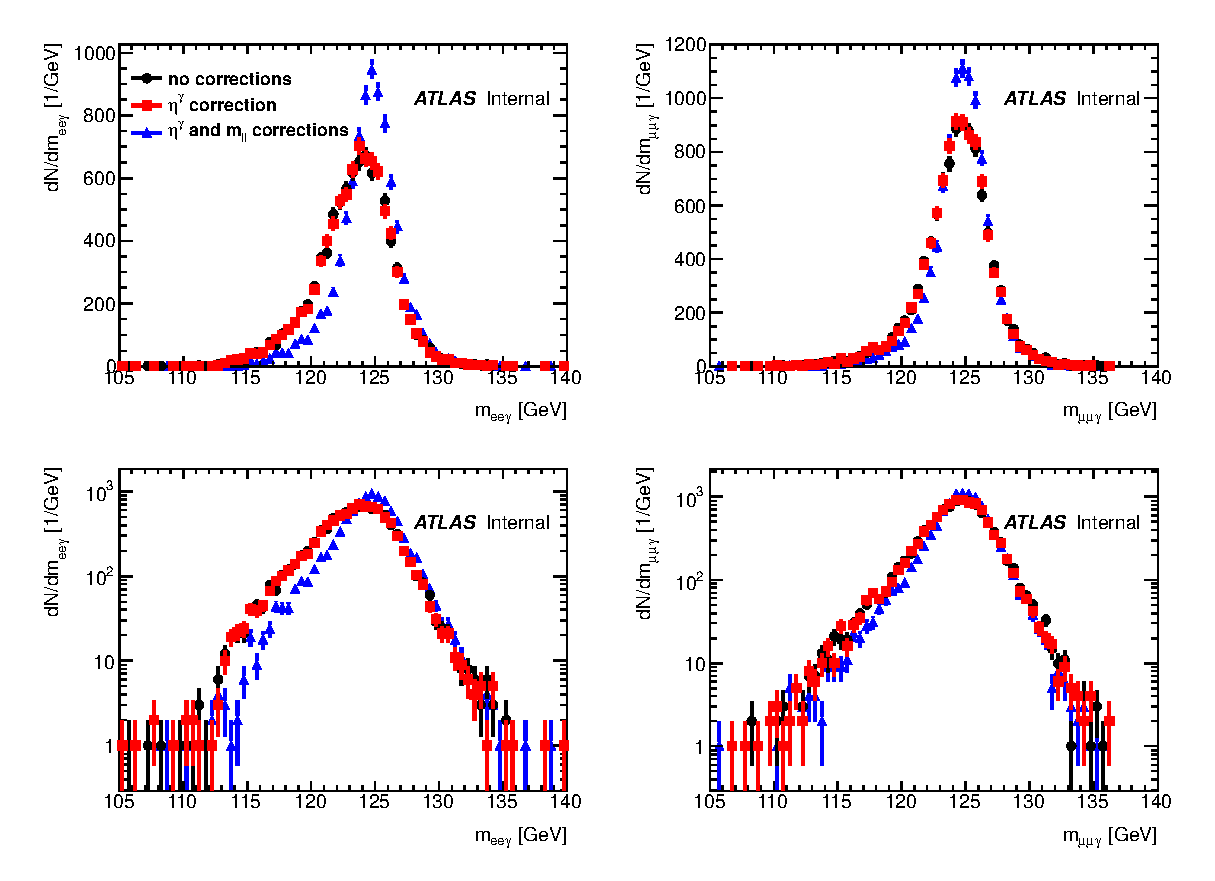
\includegraphics[width=0.99\textwidth]{figures/signal_mllg_corrections}}
{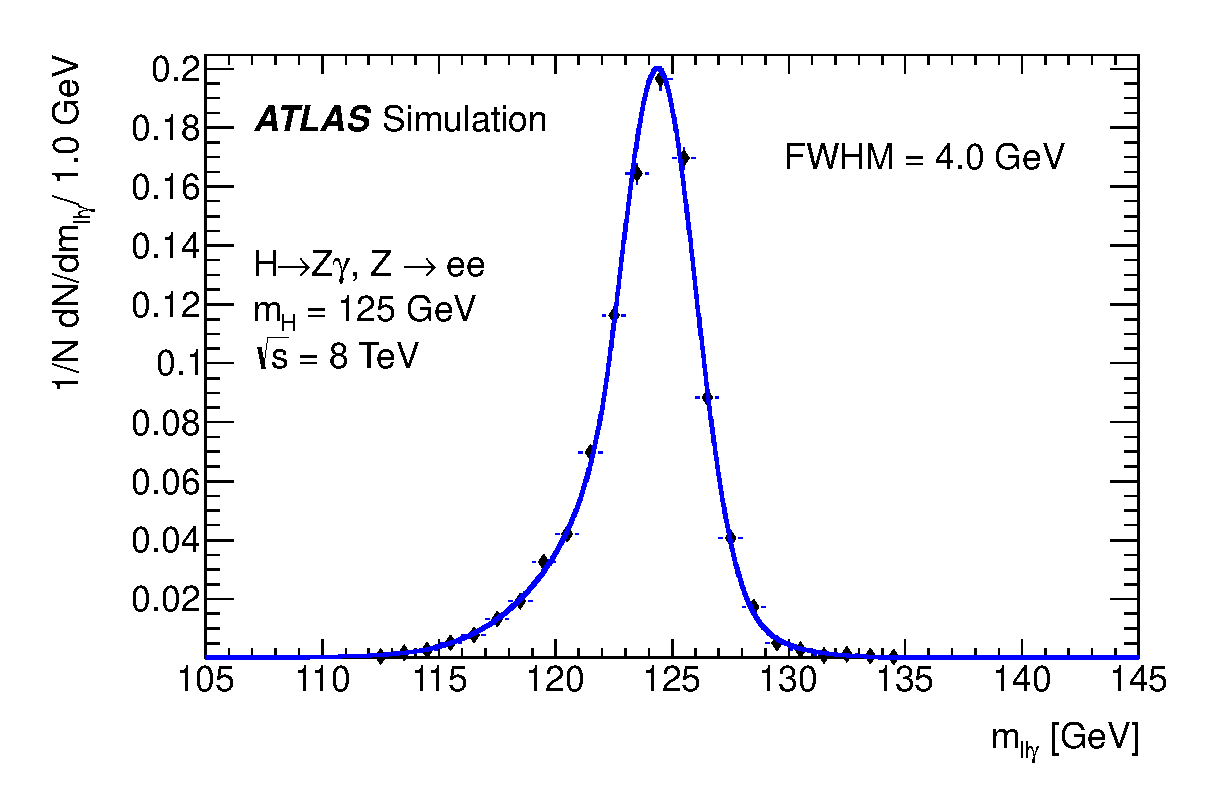
\includegraphics[width=0.48\textwidth]{figures/PlotsSuperposedResolutionCorrections_e_mc12a_Mllg}}
{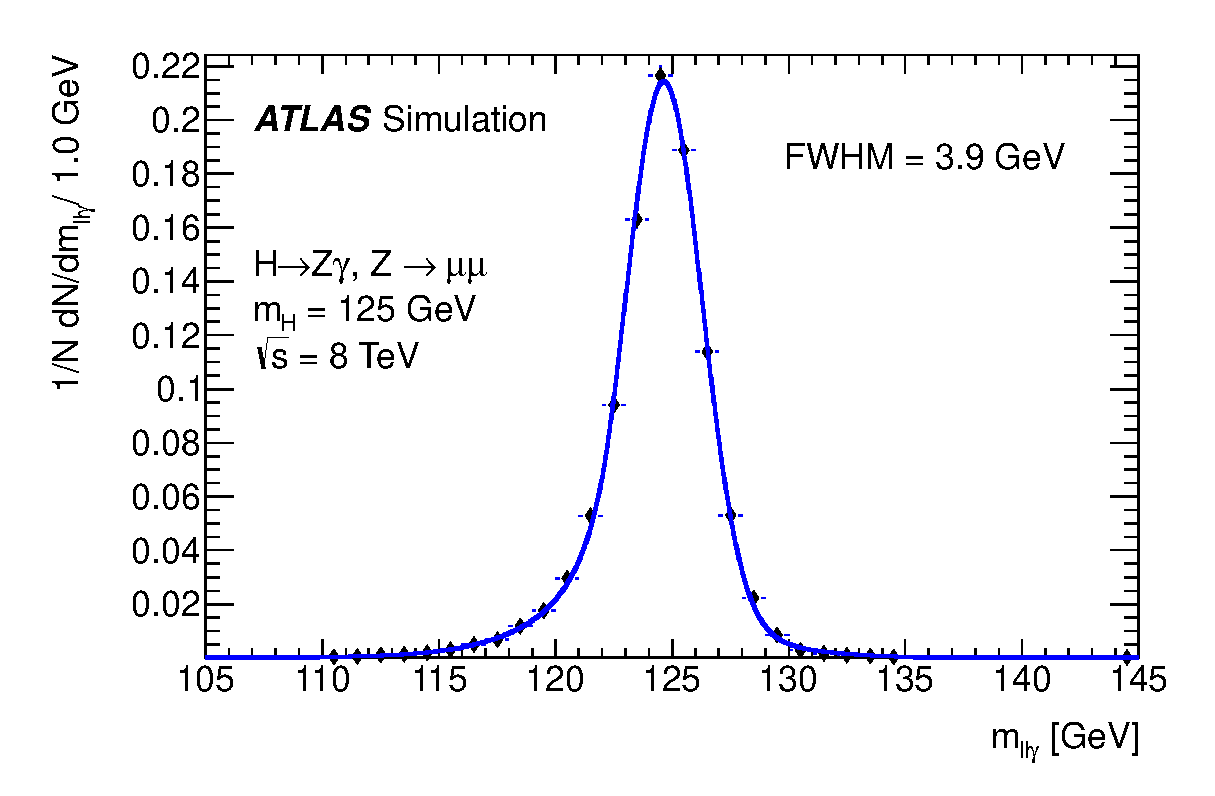
\includegraphics[width=0.48\textwidth]{figures/PlotsSuperposedResolutionCorrections_mu_mc12a_Mllg}}
\caption{Three-body invariant mass distribution for $gg\to H\to Z\gamma$
    selected events in the 8 TeV, $m_H=125$~GeV signal simulation, 
    after applying all analysis cuts and corrections. The blue solid lines 
    represent the fits to the points of the sum of a 
    Crystal Ball lineshape and a Gaussian function.
    Left: $Z\to ee$ channel, Right: $Z\to\mu\mu$ channel.}
%the standard reconstruction (red circles), and after choosing the event primary vertex as the photon origin and applying the $Z$ mass constraint to the lepton four momenta (blue diamonds). The (dashed) red line and the (blue) solid line  represent the fits to the points of the sum of a Crystal Ball lineshape and a Gaussian function. Left: $Z\to ee$ channel, right: $Z\to\mu\mu$ channel.}
  \label{fig:signal_resolution_corrections}
  \end{center}
\end{figure}

\begin{figure}[!htbp]
  \begin{center}
  {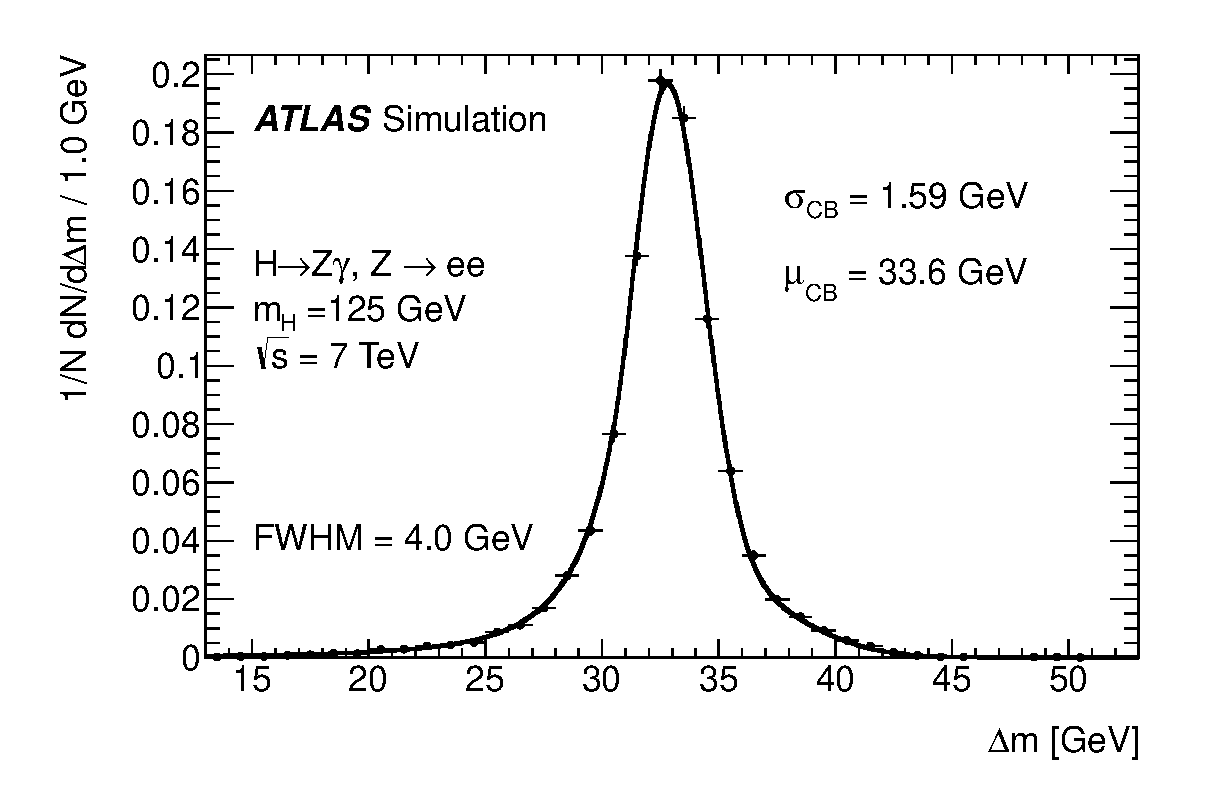
\includegraphics[width=0.46\textwidth]{figures/linPlot_125_EtaZgamma_Cat0_all_e_mc11c_mDif}}
  {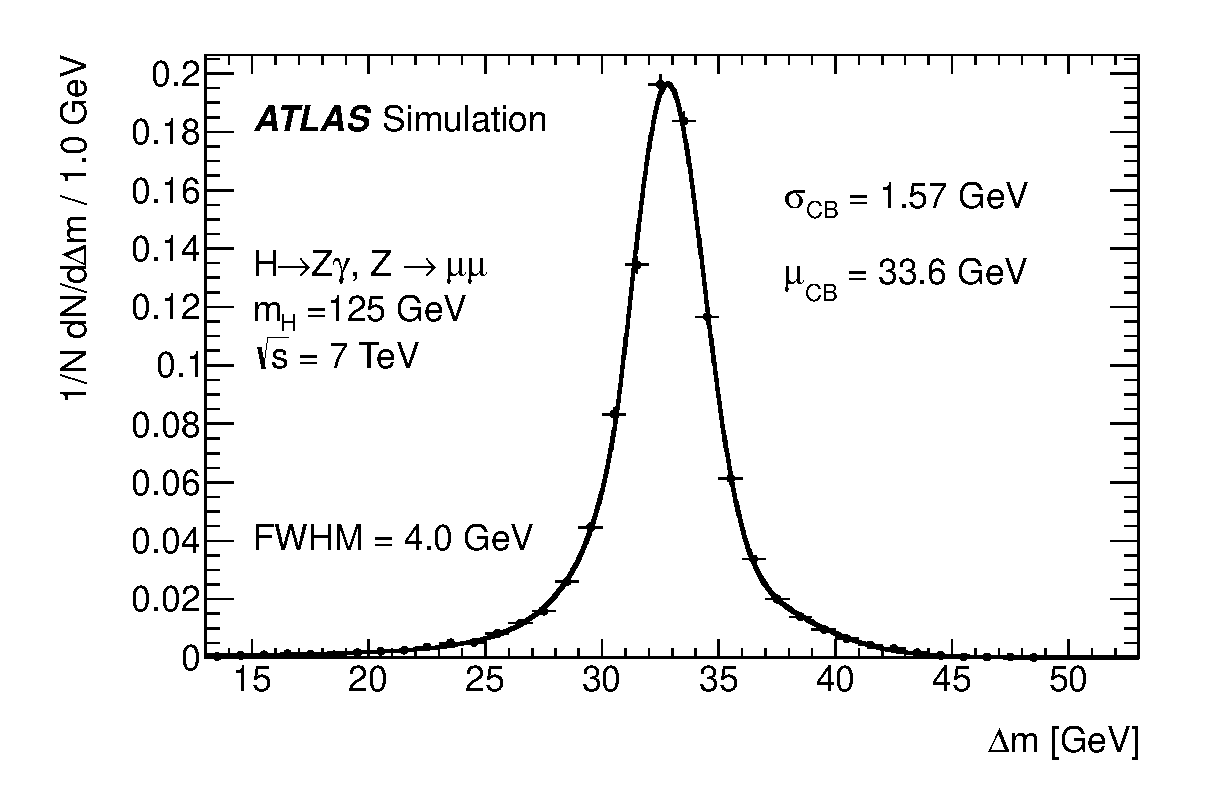
\includegraphics[width=0.46\textwidth]{figures/linPlot_125_EtaZgamma_Cat0_all_mu_mc11c_mDif}}
  {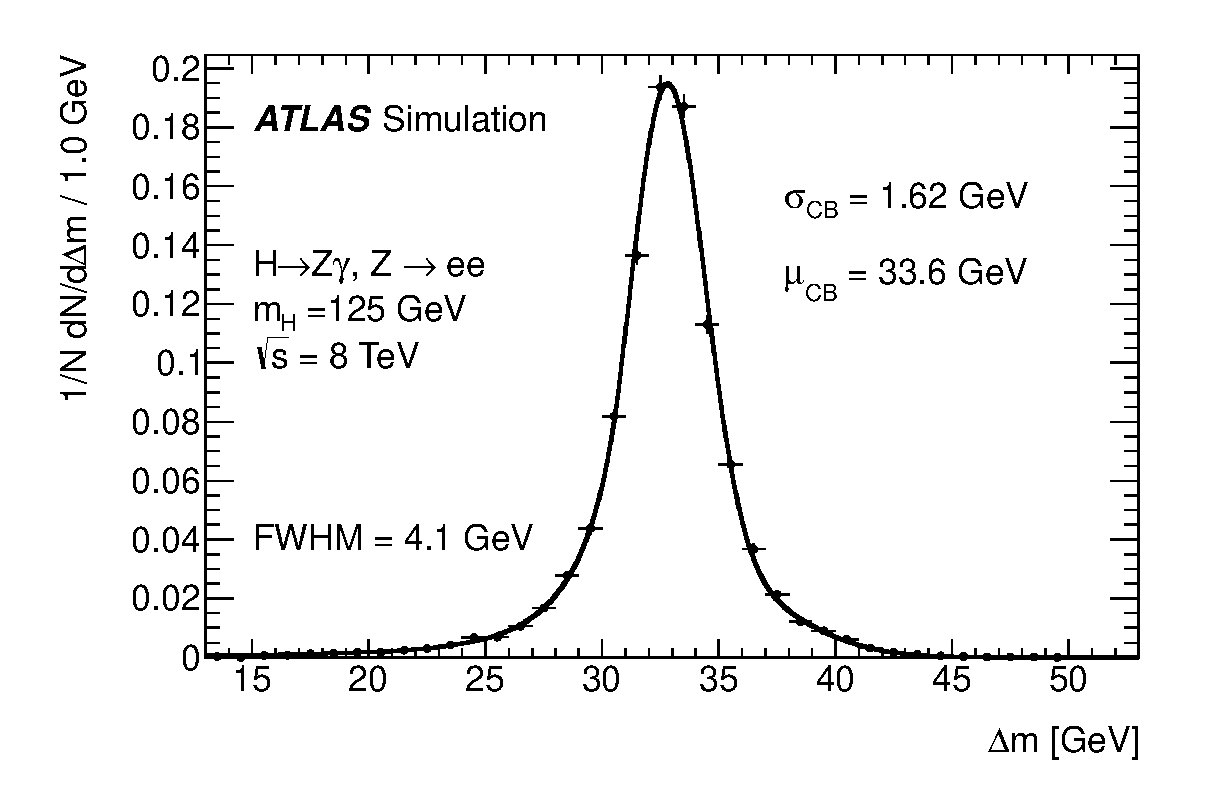
\includegraphics[width=0.46\textwidth]{figures/linPlot_125_EtaZgamma_Cat0_all_e_mc12a_mDif}}
  {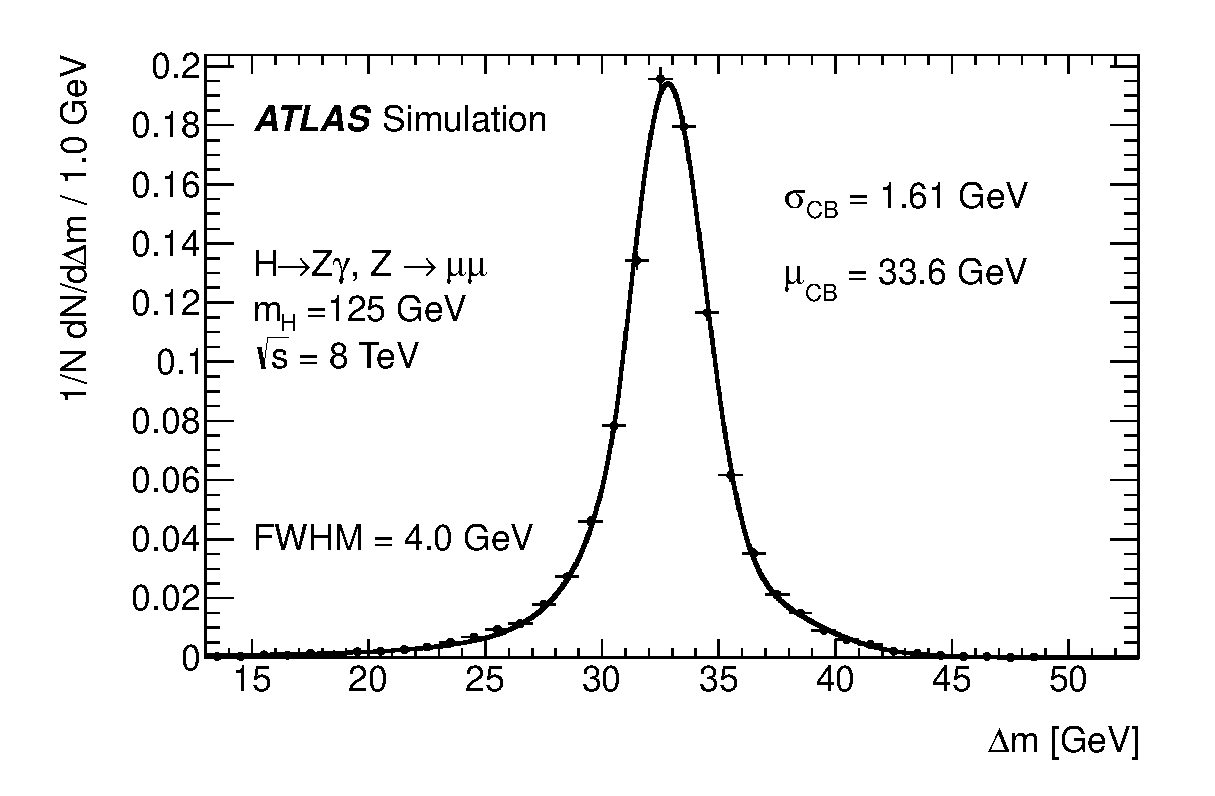
\includegraphics[width=0.46\textwidth]{figures/linPlot_125_EtaZgamma_Cat0_all_mu_mc12a_mDif}}
    \caption{Distribution (normalized to unit area) of the difference $\Delta m$ 
      between the final state three-body invariant mass
      $m_{\ell\ell\gamma}$ and the di-lepton invariant mass
      $m_{\ell\ell}$ for signal events
      passing the full selection (dots), for $m_H = 125$~GeV and $\sqrt{s}=7$ (top) or 8 (bottom) TeV. 
      The line overlaid represents the fit of the distribution with a
      model composed of the sum of a Crystal Ball (CB) and a Gaussian (GA) function.
      Left: electron channel, right: muon channel. 
    }
    \label{fig:resolution_model_example_8tev_H125}
  \end{center}
\end{figure}

